\section{Arbeit mit einer IDE}

\begin{frame}
\begin{block}{Integrierte Entwicklungsumgebungen (IDE)}
	\vspace{2pt}
	\uncover<+->{
		Die Arbeit mit gewöhnlichen Texteditoren ist auf Dauer sehr mühsam. Daher empfiehlt es sich eine IDE zu verwenden. 
		Das bringt zum u.a. folgende Vorteile: 
		\begin{itemize}[<+->]
			\item Syntax-Highlighting
			\item Code-Inspection
			\item Autocomplete
			\item Geile Shortcuts
			\item Code direkt ausführen
			\item Hilfe bei der Fehlersuche (\emph{Debugging})
		\end{itemize}	
	}
\end{block}
\end{frame}

\begin{frame}
\uncover<+->{
\begin{block}{Installation von PyCharm}
	\vspace{2pt}
	\begin{enumerate}
		\item Gehe auf 
		\texttt{https://www.jetbrains.com/pycharm/download} \\
		\item Lade die kostenlose \textit{Community Edition} herunter
		\item Führe den Installer aus
		\item Öffne PyCharm
	\end{enumerate}
\end{block}
}

\uncover<+->{
\begin{block}{Wenn alles passt, sollte es etwa so aussehen:}
	\vspace{2pt}
	\begin{center}
		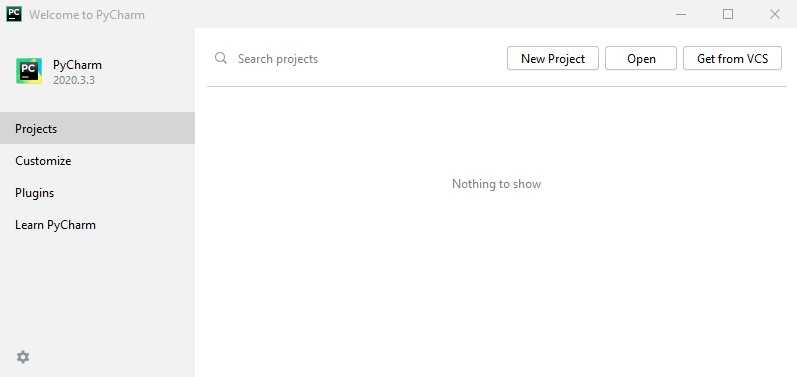
\includegraphics[width=0.65\textwidth]{pycharme.jpg}
	\end{center}
\end{block}
}	

\end{frame}








\begin{frame}
\begin{block}{Installation PyCharm}
\vspace{2pt}
\begin{enumerate}
\item Gehe auf \texttt{Customize > All Settings...}
\item Einstellungen synchronisieren
\begin{enumerate}
	\item \texttt{Tools > Settings Repository}
	\item Unter \textit{Read-only Sources} auf \texttt{+}
	\item \texttt{https://github.com/a-kunert/ide-settings.git}	eingeben
	%\item  File > Manage IDE Settings > Sync with Settings Repository > Merge ausführen 
\end{enumerate}
\item Verknüpfe den Interpreter
\begin{enumerate}
	\item In den Settings auf \texttt{Python Interpreter}
	\item Falls möglich unter \texttt{Python Interpreter} einen Interpreter wählen. Ansonsten wie folgt: 
	\item \texttt{Zahnrad > Add}
	\item \texttt{System Interpreter}
	\item Dort den Pfad zu Python angeben
\end{enumerate}
\item Mit dem Button \textit{Apply} alles bestätigen
\end{enumerate}
\end{block}
\end{frame}

\begin{frame}
\begin{block}{Konfiguration abschließen}
\begin{enumerate}
\item Lege eine Ordner für den Kurs an
\item Öffne diesen Ordner mit \texttt{Projects > Open}
\item \texttt{File > Manage IDE Settings > Sync with Settings Repository > Merge} ausführen
\item Bei \texttt{File > Settings} unter \texttt{Keymap} die Keymap \textit{Salem-Win/Mac} auswählen. 
\item Code in die Datei \texttt{main.py} schreiben
\item Mittels grünem Pfeil (oben rechts) Code ausführen
\end{enumerate}	
\end{block}
\end{frame}